\documentclass[a4paper,12pt]{article}

\usepackage[utf8]{inputenc} % spécifie l'encodage du fichier
\usepackage[english,francais]{babel} % permet de traduire les éléments latex (date, titres de sections, etc.)

\usepackage{geometry} %
\geometry{a4paper}

\usepackage{graphicx}
\usepackage{float}
\graphicspath{{tests/}}

\usepackage{array}

\usepackage[hidelinks=true]{hyperref}

\usepackage{pdfpages}
\usepackage{listings}


\usepackage{fancyhdr}
\pagestyle{fancy} 

\linespread{1.5}

\fancyhead[R]{\rightmark}
\fancyhead[L]{\leftmark}
\renewcommand{\footrulewidth}{1pt}

\begin{document}

\includepdf[pages=last-last]{dev2}

\begin{titlepage}
\selectlanguage{francais}

\newcommand{\HRule}{\rule{\linewidth}{0.5mm}}

\begin{center}

\textsc{\LARGE Programmation parallèle haute performance\\[1.5cm] 
\textsc{\Large Travail pratique \#2 - INF7235 (gr. 10)}}\\[0.5cm]
\textsc{\large Hiver 2014}\\[0.5cm] 

\HRule \\[0.4cm]
{ \huge \bfseries Parallélisation en MPI/C d'une méthode Monté Carlo appliquée à un jeux de hasard }\\[0.4cm] % Titre de votre document
\HRule \\[1.5cm]

\end{center}


\begin{minipage}{0.4\textwidth}
\begin{flushleft} \large
\emph{Auteurs:}\\
Johann \textsc{Dubois} % Nom de l'étudiant
\\
Clément \textsc{De Figueiredo}
\end{flushleft}
\end{minipage}

~~\\

\begin{center}
{\large \today}\\[3cm] % Date: \today insère la date du jour actuel

\vfill

\end{center}

\end{titlepage}
\newpage % nouvelle page

\tableofcontents % Génération du sommaire


\renewcommand\thesection{\Roman{section}}

\newpage % nouvelle page


\section{Description du problème}

"\textit{Le terme méthode de Monte-Carlo, ou méthode Monte-Carlo, désigne toute méthode visant à calculer une valeur numérique en utilisant des procédés aléatoires, c'est-à-dire des techniques probabilistes.}" \cite{wiki:montecarlo}
\\
Dans le programme élaboré dans le cadre d'un travail de session pour le cours de programmation parallèle haute performance, la méthode de Monte Carlo est appliquée aux jeux de hasard.
Plus précisément, c'est le jeu du Loto qui a été choisi afin d'y appliquer la méthode de Monte Carlo. En effet, l'objectif est de savoir quelles sont les probabilités qu'un nombre apparaisse plus qu'un autre. Dans ce but, plusieurs techniques de parallélisme ont été mise en place et leurs performances ont été mesurées afin de connaître quelle était la meilleure approche dans le contexte de la méthode de Monte Carlo appliquée au jeu du Loto. 


\section{Approches utilisées}

\subsection{Implémentation de Monte Carlo}
Le langage choisit afin d'utiliser la librairie \textbf{MPI} et le langage \textbf{C}. Ce langage a été choisi car la librairie \textbf{MPI} est compatible avec ce langage et nous disposions de connaissances suffisante en \textbf{C} afin d'implémenter cette solution de Monte-Carlo. 
\\\\Dans un premier temps, MPI est initialisé avec \textbf{MPI\_Init} puis les processus esclaves sont identifiés avec l'instruction \textbf{MPI\_Comm\_rank}. Ensuite, si le processus actuel est le processus maître alors divers opérations sont effectuées : séquentielle, parallèle statique et parallèle dynamique (sac de tâches). Chaque temps d'exécution des divers calculs sont stockés grâce à la variable \textbf{MPI\_Wtime} et sont affichés à la fin d'exécution du programme.

\subsection{Génération de nombres aléatoires}
La génération du nombre aléatoire utilisé dans la cadre de la fonction de tirage au sort a été faite de façon « Thread Safe ». C'est-à-dire que cela prévient les problèmes d'exclusion mutuelle qui pourrait avoir lieu si 2 threads voudraient récupérer une valeur, car la méthode de génération aléatoire se base sur l'horloge pour proposer un nombre.\\\\
L'utilisation de nombres aléatoires en C se fait avec les fonctions \textit{srand()} et \textit{rand()}. La première prend un argument qui servira de graine pour la génération de nombre. L'idée est alors de fournir une valeur de temps couplé avec le numéro du thread pour que la valeur soit différente pour chaque processus. \\
Le code suivant nous donne alors une valeur aléatoire « Thread Safe » : \\
\textit{srand(time(NULL) {\large \textasciicircum}  numProc);}


\subsection{Versions parallèles}

\subsubsection{Statique}
La version parallèle statique correspond à une version parallèle à granularité fine avec association statique entre tâches et threads. Autant de tâches vont être créées qu'il y a de processeurs. Chaque processus fait effectuer le tirage et les résultats vont être stockés localement. Ensuite, l'instruction \textbf{MPI\_Reduce} va avoir pour rôle d'effectuer une réduction et d'additionner (grâce à l'argument \textbf{MPI\_SUM}) tous ces résultats entre eux, le résultat final étant stocké dans un tableau final. Pour finir, on affiche les données issues du tableau récapitulatif ainsi que le temps d'exécution total. 

\subsubsection{Dynamique}
La version parallèle dynamique correspond à une version parallèle avec association dynamique entre tâches et threads de type « sac de tâches ». Cette version réalise la même opération que la version statique cependant quelques différences sont présentes. Un processus maître appelé « Coordinateur » a pour rôle de distribuer les tâches aux différents processus appelés « travailleurs ». Les « travailleurs » reçoivent les différentes tâches à effectuer avec l'instruction 

\section{Résultats expérimentaux}

\subsection{Application de test}
L'application doit être compilée et lancée avec au moins la version 4.4.7 de \textbf{gcc} (présent sur le cluster Turing de l’UQAM). Un makefile est également fourni afin d'exécuter les différentes versions du programme.\\\\
Les commandes disponibles dans le makefile sont les suivantes :
\begin{itemize}
	\item{\textbf{make compile}} (comportement par défaut de l'instruction make) pour compiler le code source
	\item{\textbf{make tests}} afin de vérifier le bon fonctionnement du programme
	\item{\textbf{make mesures}} pour exécuter le programme et en mesurer les performances
\end{itemize}~~\\
Des variables d'exécution pour également être modifiées. La variable \textbf{I} correspond au nombre total d'itérations effectués par la fonction \textbf{tirage} ainsi que la variable \textbf{NP} qui indique le nombre de processeurs utilisé par le programme.


\subsection{Conditions des tests}
Pour réaliser différents tests, plusieurs valeurs différentes vont être testées dans un environnement identique afin que les mesures soient comparables. L'application étant dépendante de la génération de nombre aléatoire, c'est pourquoi chaque mesure a été effectuée cinq fois et la moyenne de ces cinq tests a été retenue comme valeur finale. 

\subsection{Résultats}
Afin d'étudier les effets d'une implémentation parallèle, nous avions varié trois paramètres : le nombre d'itérations du tirage au sort, le nombre de threads et le nombre de tâches. \\
Dans les résultats présentés par la suite, \textit{S} correspond à « séquentiel », \textit{PS} à « parallèle statique » et enfin \textit{PD} à « parallèle dynamique ». 

\subsubsection{Variation du nombre d'itérations}
La méthode de Monte-Carlo consiste à réaliser un grand nombre de fois une opération pour que la probabilité soit élevée. Dans notre cas nous effectuons un grand nombre de fois un tirage au sort de numéros. Nous allons varier cette valeur pour comparer les différents modèles.\\

\subsubsection{Variation du nombre de threads}

\subsubsection{Variation du nombre de tâches}


\subsection{Analyse}


\section{Ouvertures}

\newpage

\nocite{*} % permet d'afficher toutes les références sans qu'elles soient citées
\bibliographystyle{unsrturl}
\bibliography{biblio}

\end{document}